\documentclass[a4paper,11pt]{article}
\usepackage[utf8]{inputenc}
\usepackage[margin=1in]{geometry}
\usepackage[english, czech]{babel}
\usepackage{amsmath}
\usepackage{csquotes}

% package na vklad obrázků
\usepackage{graphicx}
\usepackage{caption}
\usepackage{subcaption}
\usepackage{stfloats} % opravuje obrázky přes celou stránku
\graphicspath{ {./images/} } % definování složky s obrázky

% zvyšování hloubky obsahu
\setcounter{tocdepth}{4}
\setcounter{secnumdepth}{4}

% citace
\usepackage[
    citestyle=numeric,
    autocite=superscript,
    sorting=none
    ]{biblatex} 
% \usepackage{biblatex}
\addbibresource{literature.bib}

\DeclareCiteCommand{\supercite}[\mkbibsuperscript]
  {\iffieldundef{prenote}
     {}
     {\BibliographyWarning{Ignoring prenote argument}}%
   \iffieldundef{postnote}
     {}
     {\BibliographyWarning{Ignoring postnote argument}}%
   \bibopenbracket}%
  {\usebibmacro{citeindex}%
   \usebibmacro{cite}}
  {\supercitedelim}
  {\bibclosebracket}
  
% definování listings pro vklad kódu
\usepackage{listings}
\lstset{language=C++}

% abstrakt s větším písmem (https://tex.stackexchange.com/a/366170)
\makeatletter
\renewenvironment{abstract}{%
    \if@twocolumn
      \section*{\abstractname}%
    \else %% <- here I've removed \small
      \begin{center}%
        {\bfseries \Large\abstractname\vspace{\z@}}%  %% <- here I've added \Large
      \end{center}%
      \quotation
    \fi}
    {\if@twocolumn\else\endquotation\fi}
\makeatother

\selectlanguage{czech} % nastavení jazyka
\usepackage[T1]{fontenc}
% soubor k upřesnění rozdělení slov na slabiky

 % upřesnění slabik v různých cizích slovech

\begin{document}


%%% -------------------- Titulní strana --------------------
\begin{titlepage}
\begin{center}
\large \vspace*{\fill}
\thispagestyle{empty}

\LARGE

{ \huge \textbf{Gymnázium Arabská, Praha 6, Arabská 14}}

{\LARGE Obor programování }

\vfill

\includegraphics{logogyarab.png}
\vspace{15pt}

\vfill

{\huge \textbf{Fractualiser}}

\vfill

Adam Suchý

\vfill

{\large Duben, 2022}

\vspace*{\fill}
\end{center}
\end{titlepage}

%%% -------------------- Prohlášení --------------------
\thispagestyle{empty}
\addtocounter{page}{-1}
\vspace*{\fill}
Prohlašuji, že jsem jediným autorem tohoto projektu, všechny citace jsou řádně označené a všechna 
použitá literatura a další zdroje jsou v práci uvedené. Tímto dle zákona 121/2000 Sb. (tzv. Autorský zákon) 
ve znění pozdějších předpisů uděluji bezúplatně škole Gymnázium, Praha 6, Arabská 14 oprávnění k výkonu 
práva na rozmnožování díla (§ 13) a práva na sdělování díla veřejnosti (§ 18) na dobu časově neomezenou a 
bez omezení územního rozsahu.
\bigskip

V .......... dne ............... \hspace{4cm} Adam Suchý ....................
\vspace{2cm}

%%% -------------------- Anotace --------------------
\newpage
\begin{abstract}
    Fractualiser je program pro výkres fraktálů v reálném čase. Uživatel může prozkoumávat a klesat do fraktálu až
    do přiblížení $10^{13}$. Může také upravovat rovnici, podle které je fraktál vypočítáván, nebo bravy, ve kterých
    je zobrazen.
\end{abstract}

%%% -------------------- Obsah --------------------
\tableofcontents
  % povinné strany

\twocolumn
\begin{figure*}[bh!]
\centering
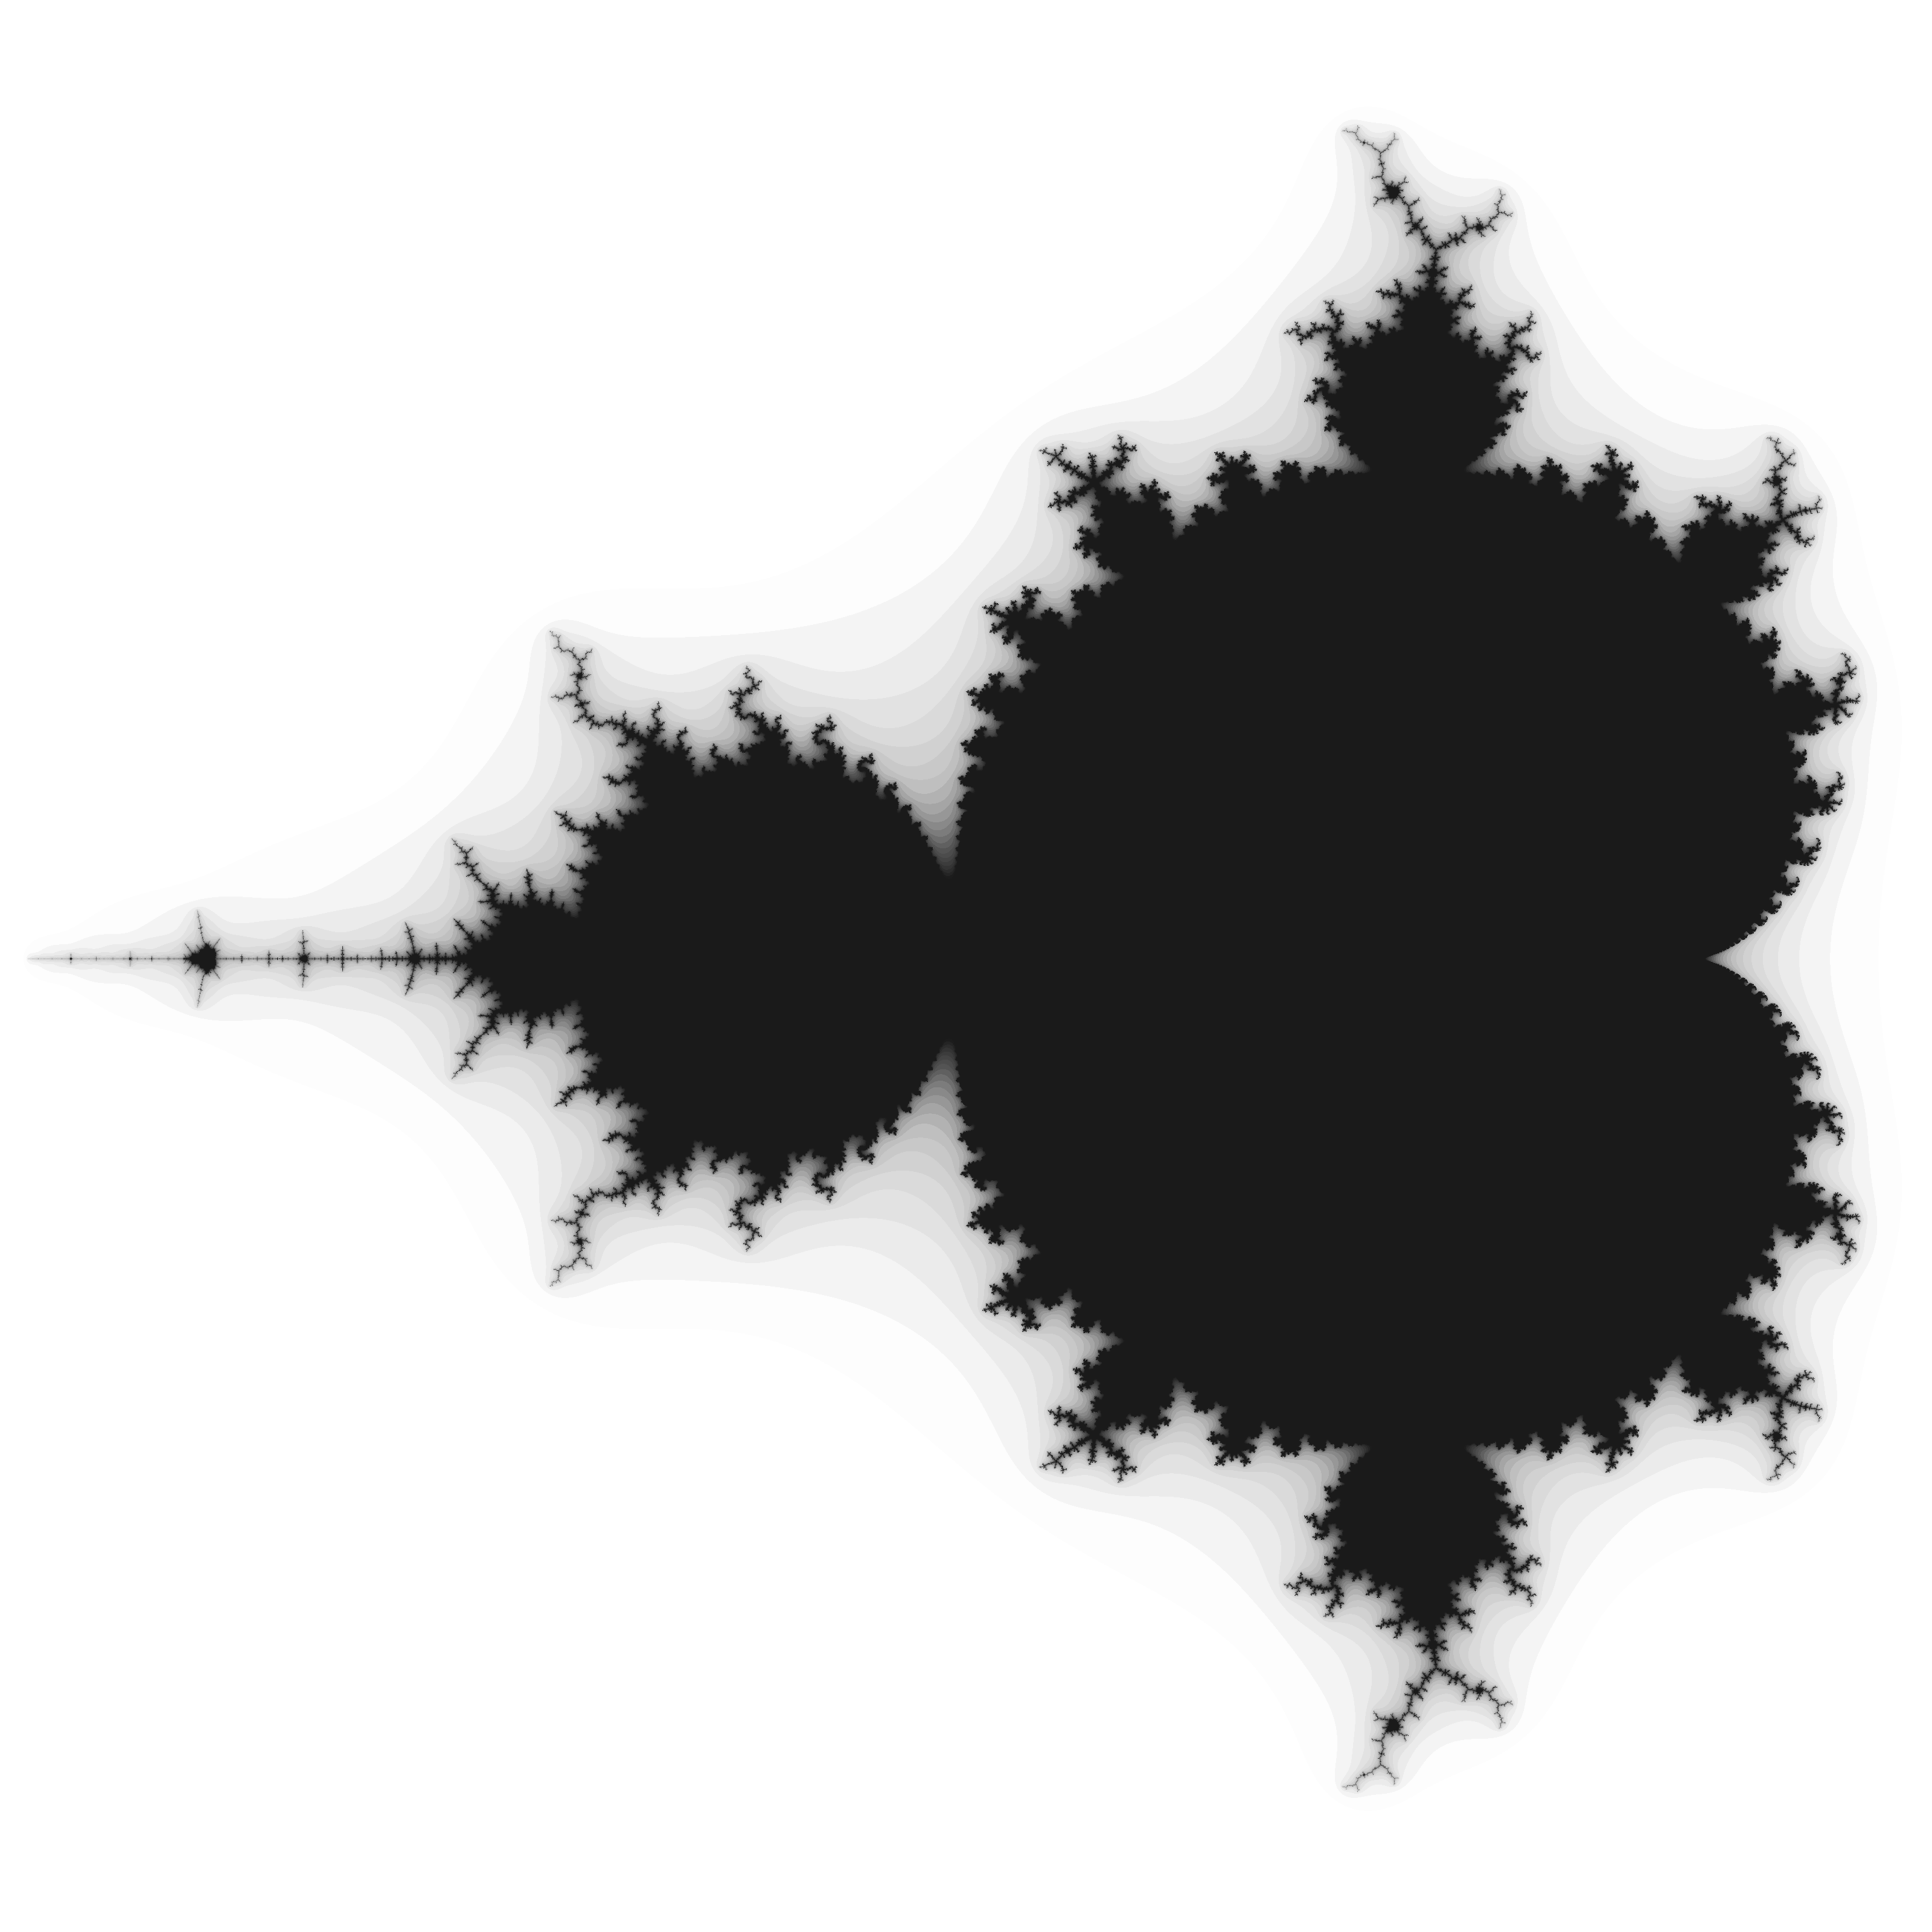
\includegraphics[width=0.6\textwidth]{mandelbrot.png}
\caption{Mandelbrotova množina}
\label{fig:mandelbrot}
\end{figure*}
\section{Úvod}
Fractualiser je program určený pro výkres fraktálů v reálném čase. Umožnujě 
tak uživatelům podbrobně prohlížet jednotlivé části až do přiblížení $10^{13}$
\footnote{Toto omezení je dáno přesností datového typu double, který dokáže
zpracovat GPU. Může se tím pádem lišit mezi počítači.}. Je v něm možné také
právě se zobrazující část fraktálu uložit ve vyšší kvalitě. Bez nastavení je
uložený obrázek čtyřikrát větší, než ten, který je zobrazovaný na obrazovce.
Uživatel ale může tuto hodnotu změnit a fraktál vygenerovat jak velký chce.
Formát uloženého obrázku je Windows Bitmap, také známý pod jeho připonou
\texttt{.bmp}. Implementace Windows Bitmap formátu byla provedena podle
\textcite{bitmapstorage}.

Fractualiser dokáže vykreslovat jen fraktály, které jsou definovány pomocí
jedné funkce v množině komplexních čísel, jako je například Mandelbrotova
množina. Mandelbrotovu množinu definujeme pomocí funkce $f_c(z) = z^2+c$, kde
$z$ a $c$ začínají jako jedno komplexní číslo, o kterém chceme zjistit, zda je
či není v množině. (obrázek \ref{fig:mandelbrot}) Funkci poté provádíme 
opakovaně. Čísla, které nikdy nepřekročí vzdálenost 3 od počátku jsou součástí
množiny.\autocite{mandelbrotwiki}

\subsection{Zadání}
Fractualiser (název složen ze slov fractal a visualiser) je program, který bude
schopen v reálném čase vykreslovat fraktály jako například Mandelbrotovu
množinu, nebo jakoukoliv z Jůliových množin. Uživatel bude moci fraktálem
pohybovat, nebo si jej přiblížit. Program mu také umožní zvýšit počet iterací
pro každý pixel, aby mohl dále klesat do fraktálu. Bude taky schopen uložit
obrázek zrovna zobrazované části fraktálu ve velkém rozlišení. Výpočet a render
bude možné zrychlit pomocí GPU akcelerace.

\subsection{Využité technologie}
Program je napsaný v programovacím jazyce C++. Hlavní důvod využití tohoto
jazyka je jeho rychlost a narozdíl od C jeho podpora objektového programování.
Na vykreslování jsem použil OpenGL API, protože je dobře podporované a
zdokumentované. Dále jsem použil nadstavbu GLFW, která zprostředkovává
zjednodušení a další abstrakce od samotného OpenGL. Na inicializaci OpenGL jsem
použil GLAD. Mi\-mo standardní knihovnu, OpenGL, GLFW a GLAD Fractualiser
nevyužívá žádné jiné kni\-hov\-ny.

Pracoval jsem v editoru NeoVim, přesněji v jeho nadstavbě LunarVim, která
poskytuje plnohodnotné IDE pomocí několika pluginů na analýzu kódu, nebo
debugování přímo v editoru. Jako debugger jsem použil GDB, což je velmi
populární debugger pro Linux, vyvíjen společností Free Software Foundation.
V několika případech byl velmi užitečný. Hlavně když program skončil
chybou SEGFAULT.

\section{Paralelizace a rychlý render}
Jeden z hlavních problémů v tomto projektu byla rychlost výpočtu zadané rovnice
pro každý pixel. Naštěstí výpočet každého pixelu je možné definovat jako čistou
funkci (anglicky pure fun\-ction)\footnote{Čisté funkce jsou funkce, které jen a
pouze vrací výsledek. Nemohou tedy např. vypsat hodnotu, nebo změnit jejich
vstup.}. Díky tomu víme, že je možné tento problém paralelizovat a jednotlivé
pixely lze bez omezení počítat současně, jelikož jeden na druhém nezávisí.

Při paralelizaci je standardně problém s orchestrací jednotlivých podprocesů,
tzn. dávání práce a získání výsledků. Naštěstí je tento problém velmi častý a
je vyřešen i pro tento specifický případ. Krom speciálního hardwaru, GPU
(Graphics Processing Unit), také existují API, které nám ho zprostředkují.

Jedno z moderních API je OpenGL. Jedná se o knihovnu, která zpřístupní
funkcionalitu GPU pomocí několika funkcí. Jazyky C++ a C sdílejí tuto samou
knihovnu, a tím pádem její používání vypadá velmi podobně v obou jazycích.
Bohužel to znamená, že nevyužívá všechny možnosti moderního C++ a OOP.

OpenGL podporuje vykreslování objektů ve 3D, což v našem případě není potřeba,
jelikož vykreslujeme jen jednu rovinu. Vykreslujeme tedy jen jeden objekt,
který pokrývá celé okno.

\subsection{OpenGL pipeline, shadery}
OpenGL render pipeline jsou kroky, co OpenGL provádí při každém renderu snímku
na obrazovce. Je definován pěti částmi, které běží na
GPU:\autocite{openglpipel}
\begin{enumerate}
    \item{Procesování vrcholů - upravuje jednotlivé vrcholy, aby dopovídaly
        např. pohledu kamery ve světě.}
    \item{Post-procesování vrcholů - další úpravy na jednotlivých vrcholech.}
    \item{Skládání vrcholů do ploch a objektů.}
    \item{Rasterizace - velmi důležitý krok u fractualiséru, jelikož se v tomto
        kroku generují výsledné pixely.}
    \item{Per-sample procesování - krok ve kterém se například míchají textury.
        Post-pro\-ce\-so\-vá\-ní jednotlivých pixelů.}
\end{enumerate}

Každý krok lze ovlivnit pomocí shaderů, což jsou programy, které běží přímo na
GPU. Při procesování vrcholů se spouští vertex shader. V našem případě je velmi
jednoduchý. Vykreslujeme jen jednu plochu a vrcholy, co zadáme k vykreslení
nemusíme nijak měnit.

\begin{figure}[h!]
\centering

\includegraphics[width=0.45\textwidth]{vrstvy.png}
\caption{Vrstvy, které vznikají při iteraci zadané rovnice}
\label{fig:vrstvy}
\end{figure}

Další z shaderů je fragment shader, který běží ve čtvrtém kroku renderovací
pipeline - rasterizaci. Toto je nejzásadnější část kódu, protože právě ta nám
umožní každý pixel na obrazovce zabarvit podle vypočítané rovnice. Tento shader
musí pro naše účely udělat několik věcí: 1. převést pozici pixelu, který počítá
na pozici v grafu, 2. spočítat, jestli bod patří do množiny a kolik iterací
bylo potřeba, abychom odhalili, že v množině není, 3. vybrat správnou barvu
výsledného pixelu z textury (tento krok je standardní ve všech fragment
shaderech). V kroku 2 bychom mohli rozhodovat čistě jen hodnotou ano či ne,
ale zapamatování si kolik iterací bylo potřeba je mnohem zajímavější a na obrázku
můžeme poté vidět jednotlivé vrstvy, jak se fraktál odhaluje (obrázek \ref{fig:vrstvy}).

\subsection{Generování shaderů}
Další z problémů, který bylo nutné vyřešit, bylo generování shader kódu ze
zadané matematické funkce. Vzhledem k tomu, že se shader musí kompilovat při
běhu programu, nebyl velký problém samotná kompilace, ale získání správného
kódu. Zvolil jsem cestu rekurzivního přepsání originální funkce na zdrojový
kód, který je poté vložen do zbytku shaderu. Zbytek shaderu je přečten ze
souboru v pracovním adresáři pod názvem \texttt{shader.glsl}. Zkušený uživatel
si tak tímto může shader upravit a generovat i jiné fraktaly, než ty, které
v tuto chvíli fractualiser podporuje.

Princip přepisu spočívá ve standarním průchodu aritmetického výrazu, jako
u vytváření aritmetického stromu. Místo vytváření uzlů ale vytváříme kusy
kódu, které poté spojíme dohromady, abychom dostali konečný výraz přepsaný
do GLSL kódu.

Jazyk GLSL standardně nepodporuje komplexní čísla, ale dokáže pracovat s
vektory. Kaž\-dé komplexní číslo je tedy znázorněno jako dvouprvkový vektor.
Kvůli tomuto omezení bylo potřeba vytvořit funkce pro násobení a dělení,
jelikož násobení vektorů není ekvivalentí násobení komplexních čísel. Sčitání a
odčítání však pro dvouprvkové vektory je.

Fukce $z*z*z + 3z - 0.2 + 0.1i$ by například po přepisu do GLSL kódu vypadala
následovně:
\texttt{mult(mult(z, z), z) + mult(dvec2(3, 0), \\z) - dvec2(0.1, 0) + dvec2(0, 0.2)}.

Fractualiser zatím podporuje jen násobení, dělení, sčítání a odčítání, ale
přidání dalších funkcí by nebyl problém. Zároveň jsou tyto operace dostatečné
na vykreslení mnoha funkcí. Jedna z optimalizací, která se nabízí, je předpočítání
konstant. Ve vygenerovaném kódu v minulém odstavci můžeme vidět, že $-0.2$ a $0.1i$
byly přepsány jako dva odlišné vektory. Přitom mohou být spojeny do jednoho:
\texttt{dvec2(-0.2, 0.1)}.

\section{Export obrázku}
Další cíl fractualiseru byla možnost vyexportovat obrázek, který může mít
několikrát větší rozlišení, než monitor uživatele. Vyexportovaný obrázek
lze poté využít například pro tisk, nebo do jiných kreativních projektů.

OpenGL vykresluje obraz do \texttt{FrameBuffer}u. Tento buffer je poté
zobrazen v okně aplikace. Abychom se vyhli limitace velikosti okna, tak
místo vykreslování do výchozího bufferu vykreslíme fraktál do textury,
kterou poté můžeme po částech číst a zapsat do souboru.

Zvolený formát exportovaného obrázku je Windows Bitmap kvůli jeho
jednoduchosti. Z tohoto samého důvodu výsledný obrázek není komprimovaný a tím
pádem může být i řádově větší než ten samý obrázek konvertovaný do formátu PNG.
Serializace do Windows Bitmap formátu byla implementována podle specifikace \\
\textcite{bitmapstorage}. Samotný formát je velmi minimalistický a jsou potřeba
jen dvě hlavičky.

\begin{lstlisting}
struct Header {
    char id[0x02] = {0x42, 0x4D};
    int file_size;
    char more_identifiers[4];
    int bitmap_start;
};
struct DIBHeader {
    int size_of_header;
    int width;
    int height;
    unsigned short num_clr_panes;
    unsigned short pixel_bitlen;
    int compression;
    int bitmap_size;
    int v_res;
    int h_res;
    int n_colors;
    int imp_colors;
};
\end{lstlisting}

\texttt{Header} slouží k identifikaci \texttt{.bmp} formátu a poté k základním
metadatům o jeho velikosti. \texttt{DIBHeader} popisuje danou bitmapu a
specifikuje detaily o jejím rozlišení, nebo barvách.

Jeden ze zvlástních problémů, který nastal při implementaci byl problém s
výchozím zarovnáním \texttt{struct}ů na 4 byty. Toto mělo ale lehké řešení a to
přidání \texttt{\#pragma pack(1)}, a\-by\-chom compiler upozornili, že nechceme, aby
tento \texttt{struct} zarovnával.

Alternativa k \texttt{.bmp} formátu by mohl být formát QOI (Quite OK Image formát),
který je velmi jednoduchý, ale zároveň dokáže obsah komprimovat skoro stejně dobře,
jako mnohem složitější PNG formát. Jediná jeho nevýhoda je špatná kompatibilita se
znamými programy.

\section{Procesování vstupu}
Fractualiser lze ovládat klávesnicí i myší. Vstup z klávesnice i myši je
nejdříve zachycen knihovnou GLFW, která nám poskytuje abstrakci od jednotlivých
API operačních systémů, nebo desktop managerů. Místo psaní toho samého kódu
několika způsoby pro Windows, X11 pro Linux, nebo pro MacOS můžeme použít GLFW
a ta nám připraví okno, ve kterém můžeme pracovat, a funkce, pomocí kterých
můžeme poslouchat příchozí vstupy od uživatele.

S myší lze obrazem pohybovat, nebo ho přiblížit či oddálit kolečkem. To samé
lze učinit pomocí kláves WASD a QE. Pomocí klávesnice můžeme vyvolat další
akce:
\begin{itemize}
    \item{\textbf{F/C} - ovládání počtu iterací. Klávesa F zvyšuje 
        maximální počet iterací pro každý pixel. Klávesa C ho snižuje.}
    \item{\textbf{G} - zobrazí informace o stavu programu}
    \item{\textbf{P} - začne export obrázku}
    \item{\textbf{ESC} - ukončí program}
\end{itemize}

GLFW nám umožňuje číst vstup vícekrát za jeden snímek. Toto je užitečné a
dovoluje nám mít rezponzivnější program. Zároveň je ale potřeba si zapamatovat
všechny vstupy do té doby, co program nevykreslí další snímek. Mimo hlavní
nastavení zobrazovaného grafu je také dočasné, které akumuluje změnu, kterou je
potřeba provést před dalším snímkem. Po každém vykreslení snímku se toto
nastavení vynuluje a následně se do něj načtou další vstupy.

\vfill\eject

\section{Kompilace}
Kompilace Fractualiseru je zaručená jen na operačním systému Linux,
Fractualiser ale nevyužívá žádných jeho specifických funkcí.
Je k ní potřeba \texttt{CMake}, compiler schopný zkompilovat C++ a
všechny dependence Fractualiseru (OpenGL, GLFW). Je potřeba také
ke knihovnám mít dostupný \texttt{CMake} toolchain soubor, aby byl 
\texttt{CMake} schopný najít knihovny pomocí \\\texttt{find\_package}.


V kořenovém adresáři zdrojového kódu spu\-sťte přes příkazový řádek
následující příkazy:
\begin{lstlisting}
$ mkdir build
$ cd build
$ cmake ..
$ make
$ cp ../src/fragment.glsl shader.glsl
$ ./fractualiser -h
\end{lstlisting}

Fracutaliser by se po posledním příkazu měl spustit a vypsat
instrukce pro jeho použití.


\newpage
\onecolumn
\printbibliography
\listoffigures

\end{document}
